\documentclass{standalone}
\usepackage{tikz}
\usetikzlibrary{shapes,arrows,positioning,fit,backgrounds,calc,matrix}

\tikzset{
    block/.style={rectangle, draw, rounded corners, 
                  minimum width=2.5cm, minimum height=0.9cm,
                  align=center, font=\small,
                  inner sep=0.1cm},
    data/.style={block, fill=blue!10},
    process/.style={block, fill=green!10},
    model/.style={block, fill=red!10},
    decision/.style={diamond, aspect=2, draw, fill=purple!10, 
                    minimum width=1.8cm, minimum height=0.8cm,
                    align=center, font=\small},
    arrow/.style={->,>=stealth,thick},
    note/.style={rectangle, draw, dashed, rounded corners,
                 fill=yellow!10, align=left, font=\footnotesize,
                 text width=4cm,
                 inner sep=0.1cm},
    phase/.style={font=\large\bfseries, text=gray!60},
    legend_item/.style={rectangle, draw, rounded corners, 
                       align=center, font=\footnotesize,
                       minimum width=3cm, % 增加宽度以适应垂直排列
                       inner sep=0.08cm}
}

\begin{document}
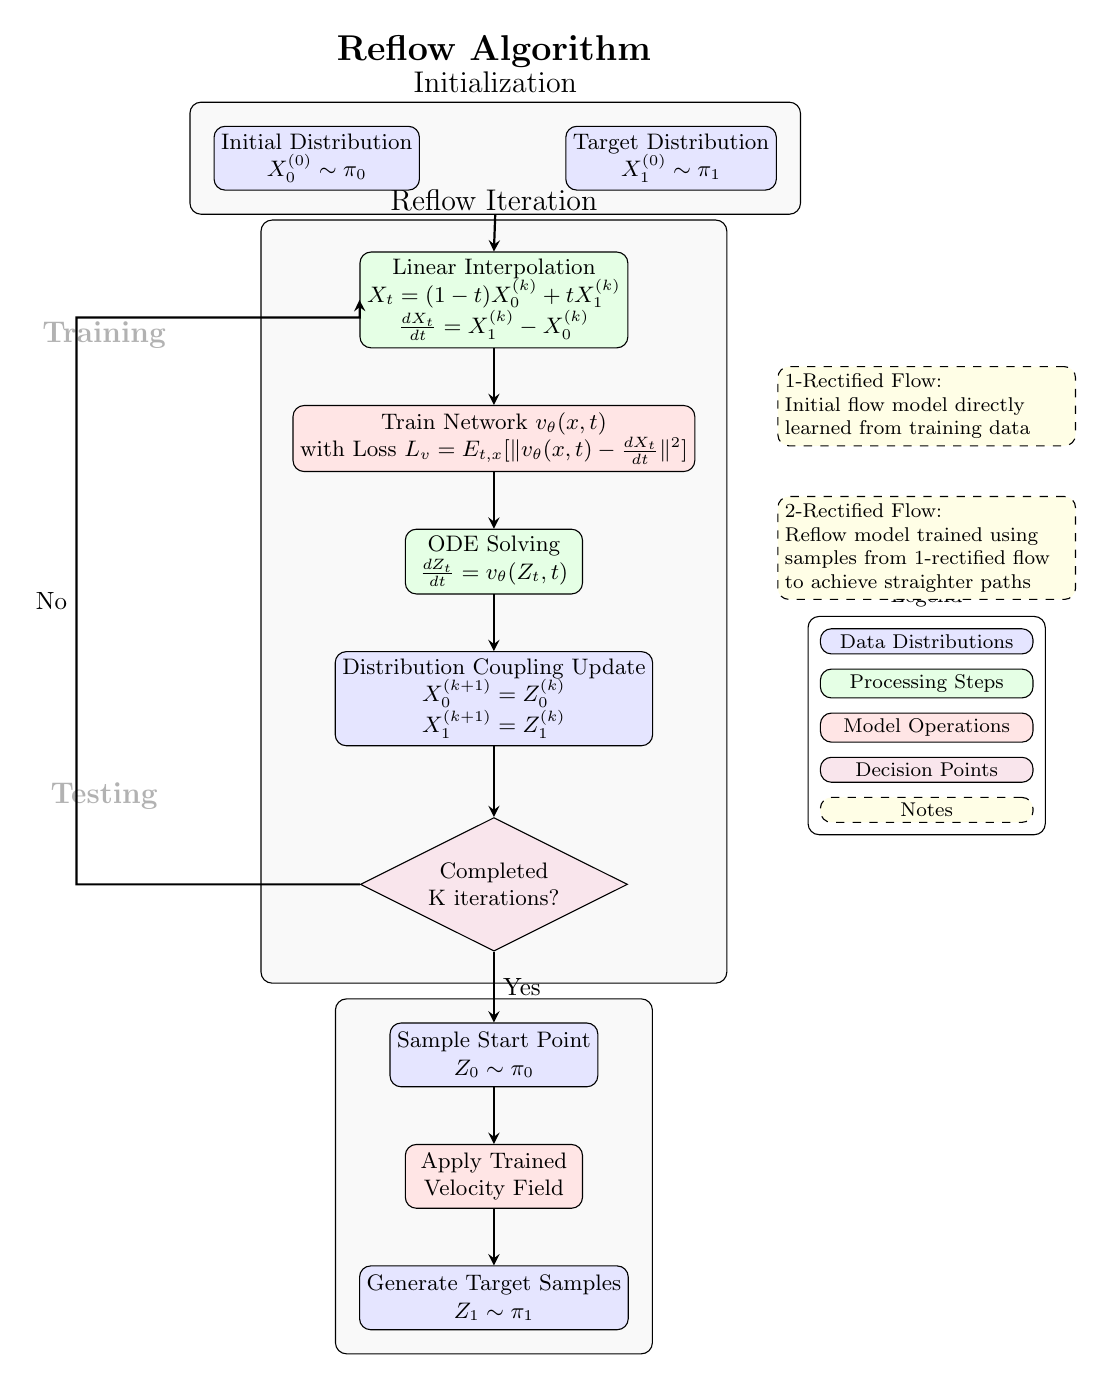
\begin{tikzpicture}[node distance=1.2cm and 4cm, scale=0.9, transform shape]
    % Title
    \node[font=\Large\bfseries] at (0,6.5) {Reflow Algorithm};
    
    % Initialization Phase
    \node[data] (init1) at (-2.5,5) {Initial Distribution\\
        $X_0^{(0)} \sim \pi_0$};
    \node[data] (init2) at (2.5,5) {Target Distribution\\
        $X_1^{(0)} \sim \pi_1$};
    
    % Background box for initialization
    \begin{pgfonlayer}{background}
        \node[fit=(init1)(init2),
              draw,rounded corners,fill=gray!5,inner sep=0.3cm] (init_box) {};
        \node[above] at (init_box.north) {\large Initialization};
    \end{pgfonlayer}
    
    % Training Phase Label
    \node[phase] at (-5.5,2.5) {Training};
    
    % Main components
    \node[process] (path) at (0,3) {Linear Interpolation\\
        $X_t = (1-t)X_0^{(k)} + tX_1^{(k)}$\\
        $\frac{dX_t}{dt} = X_1^{(k)} - X_0^{(k)}$};
    
    \node[model, below=0.8cm of path] (network) {Train Network $v_\theta(x,t)$\\
        with Loss $L_v = \mathbb{E}_{t,x}[\|v_\theta(x,t) - \frac{dX_t}{dt}\|^2]$};
    
    \node[process, below=0.8cm of network] (ode) {ODE Solving\\
        $\frac{dZ_t}{dt} = v_\theta(Z_t,t)$};
    
    \node[data, below=0.8cm of ode] (update) {Distribution Coupling Update\\
        $X_0^{(k+1)} = Z_0^{(k)}$\\
        $X_1^{(k+1)} = Z_1^{(k)}$};
    
    \node[decision, below=1cm of update] (check) {Completed\\K iterations?};
    
    % Testing Phase Label
    \node[phase] at (-5.5,-4) {Testing};
    
    % Testing Phase
    \node[data, below=1cm of check] (gen1) {Sample Start Point\\
        $Z_0 \sim \pi_0$};
    \node[model, below=0.8cm of gen1] (gen2) {Apply Trained\\Velocity Field};
    \node[data, below=0.8cm of gen2] (gen3) {Generate Target Samples\\
        $Z_1 \sim \pi_1$};
    
    % Notes
    \node[note, anchor=west] at (4,1.5) (note1) {1-Rectified Flow:\\Initial flow model directly learned from training data};
    \node[note, anchor=west] at (4,-0.5) (note2) {2-Rectified Flow:\\Reflow model trained using samples from 1-rectified flow to achieve straighter paths};
    
    % Legend - 垂直排列在右侧
    \node[legend_item, fill=blue!10, below=0.4cm of note2] (legend1) {Data Distributions};
    \node[legend_item, fill=green!10, below=0.2cm of legend1] (legend2) {Processing Steps};
    \node[legend_item, fill=red!10, below=0.2cm of legend2] (legend3) {Model Operations};
    \node[legend_item, fill=purple!10, below=0.2cm of legend3] (legend4) {Decision Points};
    \node[legend_item, fill=yellow!10, draw=black, dashed, below=0.2cm of legend4] (legend5) {Notes};
    
    % Legend box
    \begin{pgfonlayer}{background}
        \node[fit=(legend1)(legend2)(legend3)(legend4)(legend5),
              draw,rounded corners,fill=white,inner sep=0.15cm] (legend_box) {};
        \node[above] at (legend_box.north) {\small Legend};
    \end{pgfonlayer}
    
    % Connections
    \draw[arrow] (init_box.south) -- (path.north);
    \draw[arrow] (path.south) -- (network.north);
    \draw[arrow] (network.south) -- (ode.north);
    \draw[arrow] (ode.south) -- (update.north);
    \draw[arrow] (update.south) -- (check.north);
    \draw[arrow] (check.south) -- node[right] {Yes} (gen1.north);
    
    % Loop arrow
    \draw[arrow] (check.west) -- ++(-4,0) -- 
        node[left] {No} ++(0,8) -- ++(4,0) -- (path.west);
    
    % Bottom connections
    \draw[arrow] (gen1.south) -- (gen2.north);
    \draw[arrow] (gen2.south) -- (gen3.north);
    
    % Background boxes
    \begin{pgfonlayer}{background}
        \node[fit=(path)(network)(ode)(update)(check),
              draw,rounded corners,fill=gray!5,inner sep=0.4cm] (train_box) {};
        \node[above] at (train_box.north) {\large Reflow Iteration};
        
        \node[fit=(gen1)(gen2)(gen3),
              draw,rounded corners,fill=gray!5,inner sep=0.3cm] (test_box) {};
    \end{pgfonlayer}
\end{tikzpicture}
\end{document}
